\documentclass{article}

% set font encoding for PDFLaTeX, XeLaTeX, or LuaTeX
\usepackage{ifxetex,ifluatex,amsmath}
\if\ifxetex T\else\ifluatex T\else F\fi\fi T%
  \usepackage{fontspec}
\else
  \usepackage[T1]{fontenc}
  \usepackage[utf8]{inputenc}
  \usepackage{lmodern}
\fi

\usepackage{hyperref}
%Import physics package
\usepackage{physics,mathtools}
%import syntax package
\usepackage{listings, listings-rust}
%Formats URL's
\usepackage{url}
%Draw stuff
\usepackage{tikz}
%For linking to images
\usepackage{caption}

\usepackage{graphicx}
\graphicspath{ {./images/} }

\title{PWS vloeistofdynamica}
\author{Wiebe Derksen and Daniël Visser}


\begin{document}
\maketitle
\thispagestyle{empty}
\hfil
\thanks{PWS begeleiders meneer Straatman en meneer Matena, expertbegeleider Aron Van Den Bogaard}
\newpage
\tableofcontents
\newpage
%Start van het PWS zelf
\section{Introduction}
People have been simulating fluids for decades using computers, for aeronautics, movies, games and more. We thought this would be an interesting subject to write our profielwerkstuk (PWS) about because it is a quite difficult subject, but at the same time we both have a great interest in both physics and mathematics. We thought it would be easily doable but as time progressed, we started to realize this project would take quite a bit more time than we had expected. Nevertheless, it was a really interesting project. This was also the reason we decided to choose computational fluid dynamics (CFD) as the subject of our PWS.
\\ \\
Before people used computers for fluid simulations, they had to use analytical formulas. Unfortunately, the equations that describe the motion of fluids (the Navier-Stokes Equations) do not have a known analytical solution. Finding an analytical solution to the Navier-Stokes Equations is one of the Milennium Problems\cite{Millenium Problems}, the person who finds an analytical solution to the Navier-Stokes Equations will therefore get a million dollars. Although the Navier-Stokes Equations have no known analytical solution, they can be approximated numerically. Therefore, we will use a numerical approach.
\\ \\
In chapter \ref{What algorithms are feasible to implement?} \textit{What algorithms are feasible to implement?} we will discuss some common algorithms for solving the Navier-Stokes Equations and decide which algorithm we will implement, futhermore we will do some neglections to simplify the Navier-Stokes Equations and discuss boundary conditions. 
\\ \\
In chapter \ref{The implementation of the finite difference method} \textit{The implementation of the finite difference method} we will implement the finite difference method and explain our code.
\\ \\
In chapter \ref{Visualisation} \textit{Visualisation} we will explain how to render the results using Vulkan.
\\ \\
In chapter \ref{Conclusion} \textit{Conclusion} we will discuss our program and the results.


\newpage
\section{What algorithms are feasible to implement?}\label{What algorithms are feasible to implement?}
\subsection{Introduction to differential equations}
There are many algorithms to simulate liquids, each has its own advantages and disadvantages. In this chapter we will discuss these algorithms and their pro's and cons. 
\\
A differential equation can be solved either numerically or analytically. An analytical solution is a solution for the entire domain of the function. A numerical solution only gives an approximation for some discrete values.  Many differential equations are not analytically solvable, they have to be solved numerically. A numerical solution is often obtained using computers. \cite{What is discretization}




%Algorithms
\subsection{The algorithms}
%FDM
\subsubsection{Finite Difference Method (FDM)}
The Finite Difference Method (FDM) approximates the derivatives of a function using a truncated Taylor series. For a Taylor series around a point x=a the following formula applies. :\cite{Taylor series}:
\[f(x)=\sum_{i=0}^{\infty}\frac{f^{(i)}}{i!}(x-a)^{i}\]
A computer cannot keep computing forever. Therefore we have to use a truncated Taylor series. The truncated Taylor series unto i=3 is given by \cite{Taylor series approximation}
\[f(x)=f(a)+f'(a)(x-a)+\frac{f``(a)(x-a)^{2}}{2} + \frac{f^{(3)}(a)(x-a)^{3}}{6}+O(\Delta x)^{4}\]
$O(\Delta x) ^{4}$ are the truncated terms.\cite{Big O}. Using the above formula, we can calculate $f(x+\Delta x)$ by taking a=x\cite{quantstart FDM}
\begin{equation}f(x+\Delta x)=f(x)+f`(x)\Delta x + \frac{f``(x) (\Delta x)^{2}}{2}+ \frac{f^{(3)} (\Delta x)^{3}}{6} + O(\Delta x)^{4}\label{eqn:x plus deltax}\end{equation}
In the same way we can calculate $f(x-\Delta x)$:
\begin{equation}f(x- \Delta x)=f(x)-f`(x)\Delta x + \frac{f``(x)(\Delta x)^{2}}{2}-\frac{f^{(3)}(x)*(\Delta x)^{3}}{6} + O(\Delta x) ^{4} \label{eqn:x min deltax}\end{equation}
Using equation \ref{eqn:x plus deltax} we can approximate f'(x):
\[f(x+\Delta x) -f(x) = f'(x)\Delta x + O(\Delta x)^{2}\]
\[f`(x)=\frac{f(x+\Delta x) - f(x)}{\Delta x} + O(\Delta x)\]
$O(x)^{2}$ changes into $O(x)$ if it is divided by $\Delta x $. The equation above is called a first order approximation, because the lowest power in the big O is 1. The lowest power of the big O of a second order approximation is 2. $O(\Delta x)^{n}$ decreases to zero when $\Delta x$ becomes smaller, because $O(\Delta x)^{n}$ consists only of powers of $\Delta x$. The higher the lowest power, the faster $O(\Delta x)^{n}$ declines and the better the derivative is approximated. We can calculate the second order approximation using equations \ref{eqn:x plus deltax} and \ref{eqn:x min deltax}
\begin{equation}f'(x)=\frac{f(x+\Delta x)-f(x-\Delta x)}{2\Delta x}\label{taylor deriative}\end{equation}
We can also use \ref{eqn:x plus deltax} and \ref{eqn:x min deltax} to calculate the second approximation of the second derivative.
\begin{equation}f''(x)=\frac{f(x+\Delta x)-2f(x)+f(x-\Delta x)}{(\Delta x)^{2}} \label{second derivative} \end{equation}
Equation \ref{taylor deriative} can be used to turn a differential equation into an equation without derivatives, which is much easier to solve.
%TODO: check whether they are linear or not -WD
%FEM
\subsubsection{Finite Element Method (FEM)}
The Finite Element Method(FEM) is commonly used to solve differential equations. It has a lot of applications, CFD (Computational fluid dynamics) being only one of them. Unlike the FDM the FEM does not solve the equations for only a few points, but for the entire domain. It does so by approximating the differential equation with linear subfunctions. The linear subfunctions will have unknown coefficients. These coefficients are put into a matrix.
%FVM
\subsubsection{Finite Volume Method(FVM)}
The finite volume method calculates the movement of "fluid particles". These particles are discretized points of a certain volume.\cite{Finite Volume} Therefore the FVM gives the exact expression for the average value of the solution (over the hence described volume). %For each volume there is a flow in (Diffusion), %a flow out (Convection), a transient term(the disturbance of the %volume) and a source term resulting in the formula below.
%\[\pdv{\rho\phi}{t} + \nabla \cdot (\rho\boldsymbol{v}\phi) = %\nabla \cdot (\Gamma^\phi\nabla\phi) + Q^\phi\]
%Spectral Element method
\subsubsection{Spectral Element Method}
The spectral element method is a solution to the partial differential equation derived from the finite element method.
%Latice Boltzmann Method
\subsubsection{Lattice Boltzmann Method}
The Lattice Boltzmann Method models liquids as if the liquid exists of an n number of fictive particles. The method divides the simulation into two interchanging steps, collision and streaming. The steps change the density $\rho{(\vec{x},t)}$ at position $\vec{x}$ at time t. Because the Lattice Boltzmann method works within a lattice (a grid with an n amount of points in an m number of dimensions), you can draw up a formula $f_{i}(\vec{x},t)$. In this formula $f_{i}$ is the the influence of a neighbouring point i on $\vec{x}$ (a point on the lattice). The movement vector in a point then becomes: \[P_{i}(\vec{x},t) = \sum_{i=0}^{a}f_{i}(\vec{x},t)\] Where a is the number of adjacent points on the lattice and P the movement of the particle.
\paragraph{Collision} %Misschien handig om uit te leggen wat een lattice is. 
For simulating the collision of particles within the lattice, the formula is \cite{Lattice Boltzmann implementation}:
\[f_{i}(\vec{x}, t + \delta_t) = f_{i}(\vec{x}, t) + \frac{f_{i}^{eq}(\vec{x},t) - f_{i}(\vec{x},t)}{\tau_{f}}\]
$f_{i}(\vec{x}, t + \delta_t)$ is the influence at time $t + \delta_t$ with $\delta_t$ the size of the time step. A smaller $\delta_t$ leads to a more accurate simulation, but also leads to more computing time required to simulate a certain situation. \\
$\tau_{f}$ is a constant that depends on the viscosity of the simulated liquid. $f_{i}^{eq}(\vec{x},t)$ is the equilibrium density.
\paragraph{Streaming}
For simulating the actual movement of the particles the formula is: 
\[f_{i}(\vec{x}+\vec{e_i},t + \delta_t) = f_{i}(\vec{x},t)\]
Here $f_{i}(\vec{x}+\vec{e_i},t + \delta_t)$ is the fluid density at point $\vec{x}$ and $\vec{e}$ is the movement vector (the change in perceived density) of the density.
%Boundary Element Method
\subsubsection{Boundary Element Method}
The boundary element method is a method of simulating fluid dynamics with the presence of an influence of the boundary of the simulation, on the simulation. For this reason the boundary element method is quite complex and not really in the scope of this project. \cite{Boundary Element Method}
%Turbulence Methods
\subsubsection{Turbulence methods}
Apart from the above mentioned methods, there are also turbulence methods. These methods are able to simulate turbulent flows of liquids. These methods use a huge amount of computing power and thus are not really feasible for this paper.
%Some Choices
\subsection{Some Choices}
Due to the finite difference method being relatively easy to implement, we have decided to start by implementing that method. For a programming language we have chosen (provisionally) for Rust \cite{Rust} (the programming language) as it is fast and reasonably easy.
%Neglections
\subsection{Neglections in the Navier-Stokes Equations}
\subsubsection{The dimension}
It is easier for computers to solve a 2D problem than a 3D problem, because for a 2D problem the number of grid points is smaller then for a 3D problem. For example, a 10 by 10 grid contains 100 points, while a 10 by 10 by 10 grid contains 1000 points. Furthermore, 2D rendering is easier then 3D rendering. However, nowadays computers are very fast. Therefore, our computers will be able to solve 3D problems. Since we intend to simulate a container with water, we will do a 3D simulation.
\subsubsection{Compressible and incompressible Navier-Stokes Equations}
All fluids can be compressed. Their volume gets smaller when the pressure on the gas or liquid increases. However, in many cases the change in volume is not significant therefore the flows can then be approximated as incompressible flows. The Navier-Stokes Equations can be simplified to the incompressible Navier-Stokes Equations when a fluid is not compressible. Water is not very compressible\cite{NSE features}, so we will use the incompressible Navier-Stokes Equations. The incompressible Navier-Stokes equations for a Newtonian fluid, such as water, are:\cite{Navier Stokes incompressible} \cite{NASA NSE}
\begin{equation}
\begin{aligned}
&\pdv{v_{x}}{x}+\pdv{v_{y}}{y}+\pdv{v_{z}}{z}=0\\
&\left(\frac{\partial v_{\mathrm{x}}}{\partial t}+\frac{\partial v_{\mathrm{x}}}{\partial x} v_{\mathrm{x}}+\frac{\partial v_{\mathrm{x}}}{\partial y} v_{\mathrm{y}}+\frac{\partial v_{\mathrm{x}}}{\partial z} v_{\mathrm{z}}\right) \rho=-\frac{\partial p}{\partial x}+\eta\left(\frac{\partial^{2} v_{\mathrm{x}}}{\partial x^{2}}+\frac{\partial^{2} v_{\mathrm{x}}}{\partial y^{2}}+\frac{\partial^{2} v_{\mathrm{x}}}{\partial z^{2}}\right)+\rho g_{\mathrm{x}}\\
&\left(\frac{\partial v_{\mathrm{y}}}{\partial t}+\frac{\partial v_{\mathrm{y}}}{\partial x} v_{\mathrm{x}}+\frac{\partial v_{\mathrm{y}}}{\partial y} v_{\mathrm{y}}+\frac{\partial v_{\mathrm{y}}}{\partial z} v_{\mathrm{z}}\right) \rho=-\frac{\partial p}{\partial y}+\eta\left(\frac{\partial^{2} v_{\mathrm{y}}}{\partial x^{2}}+\frac{\partial^{2} v_{\mathrm{y}}}{\partial y^{2}}+\frac{\partial^{2} v_{\mathrm{y}}}{\partial z^{2}}\right)+\rho g_{\mathrm{y}}\\
&\left . \left(\frac{\partial v_{\mathrm{z}}}{\partial t}+\frac{\partial v_{\mathrm{z}}}{\partial x} v_{\mathrm{x}}+\frac{\partial v_{\mathrm{z}}}{\partial y} v_{\mathrm{y}}+\frac{\partial v_{\mathrm{z}}}{\partial z} v_{\mathrm{z}}\right) \rho=-\frac{\partial p}{\partial z}+\eta\left(\frac{\partial^{2} v_{\mathrm{z}}}{\partial x^{2}}+\frac{\partial^{2} v_{\mathrm{z}}}{\partial y^{2}}+\frac{\partial^{2} v_{\mathrm{z}}}{\partial z^{2}}\right)+\rho g_{\mathrm{z}}\right .
\end{aligned}
\label{NSE incompressible}
\end{equation}
The equation at the top is called the continuity equation. The others are the momentum equations. The spatial derivatives of the left hand side are called the convection terms. The parts on the right hand side between brackets are called the diffusion terms. The parts involving pressure are the pressure terms and \(\rho g\) is the gravitational force.
\subsubsection{Viscosity}
All fluids have viscosity. But, like compressibility, it can be neglected sometimes. Viscosity is: \(\eta=\frac{F/A}{dv_{x}/dz }\). Here F is the shear force, that is the force parallel to a surface. A is the surface and \(dv_{x}/dz\) is the change in velocity.\cite{Viscosity}. We will not neglect viscosity, because we do intend to simulate a water container with boundaries and viscosity is important near boundaries, because there is dissipation over there.\cite{NSE features} Dissipation is the conversion of some form of energy to heat energy\cite{Dissipation}. Without viscosity the Navier-Stokes Equations reduce to the Euler Equations\cite{NSE features}.
\subsubsection{Laminar and Turbulent flows}
Flows can be either laminar or turbulent\cite{NSE features}. In laminar flows there is no disruption between adjacent layers, but in turbulent flows there is. Turbulent flows have chaotic paths and they swirl. The Navier-Stokes Equations for laminar and turbulent flows are the same. But there are very small changes in pressure, velocity and temperature in turbulent flows, which should be dealt with. Although a turbulent flow can be modelled using the Navier-Stokes Equations, this costs a lot of computation power due to small changes.\cite{Turbulence} Therefore, they are often modelled in another way. The simulation of turbulent flows is beyond the scope of this project.
\subsubsection{Steady and unsteady} \label{(un)steady}
A flow is either steady or unsteady\cite{NSE features}. In a steady flow parameters, such as velocity, do not change over time. In a unsteady flow parameters can change over time.\cite{Steady and unsteady} We will simulate a unsteady flow, because we want the water in the container to be able to move.
%Boundary conditions
\subsection{Boundary conditions}
To solve a partial differential equation it is necessary to enforce boundary conditions. A container with water has two types of boundaries. One type are the walls and the floor. The other is the free surface of the water. The free surface is the surface where the water and air touch each other. The boundary condition at the free surface is trickier than that at the walls and floor, since the free surface can move, while the walls and floors can not. 
\subsubsection{No-slip boundary condition} \label{no-slip boundary condition}
The no-slip boundary condition supposes the velocity of a fluid that touches a solid is equal to the velocity of the solid \cite{no-slip boundary condition}.
\subsubsection{Free slip boundary condition}
The free-slip boundary condition presumes the velocity of the fluid perpendicular to the wall is zero, so the fluid can not move through the wall. But it does not restrict the velocity parallel to the wall.\cite{free slip boundary condition} 
\subsubsection{Dynamic boundary condition}
The dynamic boundary condition assumes the pressure on the free surface must be constant.
\newpage
%Programming
\section{The implementation of the finite difference method} \label{The implementation of the finite difference method}
\subsection{Constants} \label{Constants}
First, we define some constants. We have not taken significance into account, because we sometimes needed to add more zeros to prevent errors. These errors happen because Rust only wants f32's as decimal numbers, although they can end with .0 .
\begin{lstlisting}[language=Rust, style=boxed, breaklines=true]
///Physical constants
const GRIDELEMENTSCALE: f32 = 0.05;//The size of a grid element in meters(denoted in equations as delta x)
const TIMESTEPSIZE: f32 = 0.0005;//The size of a time step size in seconds
const DENSITY: f32 = 997.0;//Density of the liquid in kg/m^{3}. We simulate water.
const EXTERNALFORCE : [f32; 3] = [0.0,0.0,-9.81];//Gravity in N
const VISCOSITY: f32 = 0.001;//Viscosity in Pa*s.
const ATMOSPHERIC_PRESSURE: f32=101.325;//Atmospheric pressure in Pa

const MAXITERATIONSPERTIMEFRAME:i32=200;//This constant sets a maximum so the computer can not get in an infinite loop.
const RELEXATION: f32=1.0;//Pressure correction is often underestimated, this factor should be between 1.4 and 1.8.
const ALLOWEDERROR: f32=0.000001; 

//Pressure is measured in Pascal, because it is the standard SI unit for pressure.

//Grid size(e.g. number of elements in each dimension)
const PRESSUREGRIDSIZE: [usize; 3] = [10,10,10];//x,y,z
\end{lstlisting}
\newpage
\subsection{Odd-even decoupling} \label{odd-even}

%Image
\begin{figure}[h]
\centering
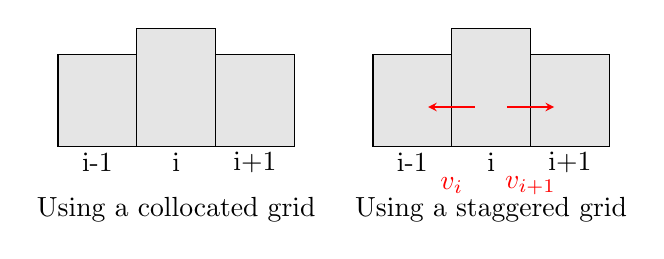
\begin{tikzpicture}
%Collocated grid
\filldraw[fill=black!10!white, draw=black] (0,0) rectangle (1,1.168);
\node[] at (0.5,-0.2) {i-1};
\filldraw[fill=black!10!white, draw=black] (1,0) rectangle (2,1.5);
\node[] at (1.5,-0.2) {i};
\filldraw[fill=black!10!white, draw=black] (2,0) rectangle (3,1.168);
\node[] at (2.5,-0.2) {i+1};
\node[] at (1.5,-0.8) {Using a collocated grid};
%Staggered grid
\filldraw[fill=black!10!white, draw=black] (4,0) rectangle (5,1.168);
\node[] at (4.5,-0.2) {i-1};
\filldraw[fill=black!10!white, draw=black] (5,0) rectangle (6,1.5);
\node[] at (5.5,-0.2) {i};
\filldraw[fill=black!10!white, draw=black] (6,0) rectangle (7,1.168);
\node[] at (6.5,-0.2) {i+1};
\draw [red, stealth-] (4.7, 0.5) -- (5.3, 0.5);
\draw [red, -stealth] (5.7, 0.5) -- (6.3, 0.5);
\node[red] at (5,-0.5) {\(v_{i}\)};
\node[red] at (6,-0.5) {\(v_{i+1}\)};
\node[] at (5.5,-0.8) {Using a staggered grid};
\end{tikzpicture} \caption{Collocated and staggered grids} \label{Odd-even decoupling} \end{figure}
%Odd-even decoupling
The Finite Difference Method calculates the pressure and velocity at discrete grid points. We can choose ourselves which variables will be calculated at which points. It would be the most easy to store all variables at every point. Such a grid is called a collocated grid\cite{Staggered grid}. However, as figure \ref{Odd-even decoupling} shows, there will be no fluid flow between cell i-1 and i and cell i and i+1 when the pressure in cells i-1 and i+1 is equal in such a grid. This phenomenon is called odd-even decoupling and happens because the derivative in cell i will be zero\cite{Staggered grid}. It is so called because information from odd and even cells are not combined properly\cite{Staggered grid}. To solve this problem we will use a staggered grid, such as in the right side of figure \ref{Odd-even decoupling}. A staggered grid consists of cells. The pressure is stored in the cell center and the velocities in the cell edges that are perpendicular to them\cite{Staggered grid}. As one can see, the derivatives will not be zero anymore, since the flow between two cells will not depend on the pressure in other cells anymore.
\newpage
\subsection{Boundary conditions and walls} \label{Boundary conditions and walls}
\begin{figure}[ht]
% body of the figure
\centering
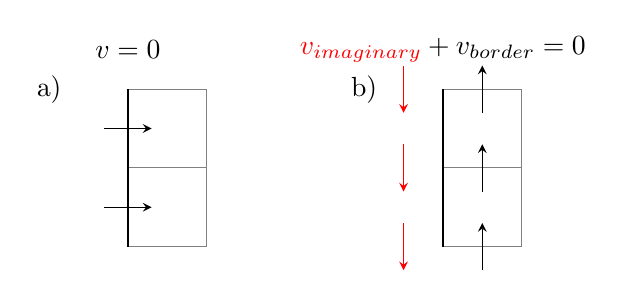
\begin{tikzpicture}
\draw[step=1cm,gray,thin] (0,0) grid (1,2);
\draw [thick] (0,0) -- (0, 2);
\draw [-stealth] (-0.3,0.5) -- (0.3, 0.5); 
\draw [-stealth] (-0.3,1.5) -- (0.3, 1.5);
\node[] at (0, 2.5) {$v=0$};
\node[] at (-1, 2) {a)};

\draw[step=1cm,gray,thin] (4,0) grid (5,2);
\draw [thick] (4,0) -- (4, 2);
\draw [-stealth] (4.5,-0.3) -- (4.5, 0.3); 
\draw [-stealth] (4.5,0.7) -- (4.5, 1.3);
\draw [-stealth] (4.5,1.7) -- (4.5, 2.3);
\node[] at (3, 2) {b)};

\draw [stealth-, red] (3.5,-0.3) -- (3.5, 0.3); 
\draw [stealth-, red] (3.5,0.7) -- (3.5, 1.3);
\draw [stealth-, red] (3.5,1.7) -- (3.5, 2.3);

\node[] at (4, 2.5) {$\textcolor{red}{v_{imaginary}}+v_{border}=0$};

\end{tikzpicture}

\caption{Wall boundary conditions} \label{wall boundary conditions}
\end{figure}

The water container is surrounded by walls on all sides.  We will use no-slip boundary conditions at the walls, as discussed in paragraph \ref{no-slip boundary condition}\cite{MAC}. This means the velocities of the water at the wall will be equal to the velocity of the wall. The wall velocity is always zero, so the velocity of the water is zero at points on the wall. Therefore, all velocity components should be zero for wall points\cite{MAC}. Unfortunately, as can be seen in figure \ref{wall boundary conditions}.a only the velocity perpendicular to the wall has points that are at the wall. However, by using an imaginary velocity outside the box we can obtain the velocity at the wall using the average\cite{MAC}:
\[v_{wall}=\frac{v_{imaginary}+v_{border}}{2}\]
Here v is parallel to the wall (so not necessarily in the y-direction), \(v_{wall}\) is the velocity at a wall point, \(v_{border}\) is the velocity that is closest to the certain wall point and \(v_{imaginary}\) is the imaginary velocity. We can modify the formula to obtain \(v_{imaginary}\) quite easily:
\[\begin{split}
&v_{wall}=0\\
&=>\frac{v_{imaginary}+v_{border}}{2}=0\\
&=>v_{imaginary}+v_{border}=0\\
&=>v_{imaginary}=-v_{border}\\
\end{split}\]
Because of the imaginary velocity grid points, we will have to make the grid larger in some directions.\\ \\

In short, we have the following boundary conditions: \\
1) The velocities on the edge of the box that are perpendicular to the edge of the box are zero.\\
2) The imaginary velocities are equal to the additive inverse of the velocities opposite of the wall.

\newpage
\subsection{The sizes of the grids} \label{The sizes of the grids}
\begin{figure}[ht]
\centering
% body of the figure
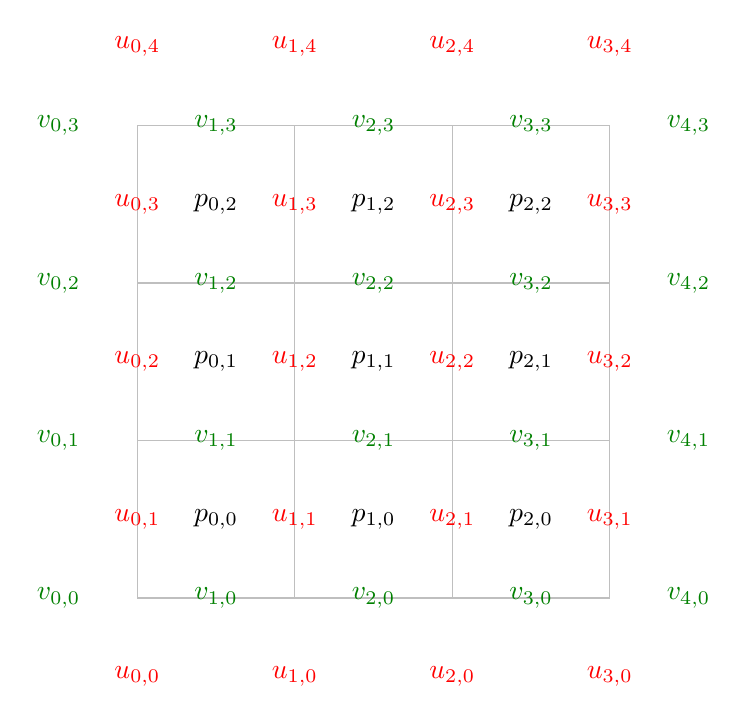
\begin{tikzpicture}
\draw[step=2cm,gray!50!white,thin] (0,0) grid (6,6);

\foreach \x in {0,1,2}
  \foreach \y in {0,1,2}
    \draw (2* \x cm + 1cm, 2* \y cm + 1cm) node[] {$p_{\x, \y}$};

\foreach \x in {0,1,2,3}
  \foreach \y in {0,1,2, 3, 4}
    \draw[red] (2* \x cm, 2* \y cm - 1cm) node[] {$u_{\x, \y}$};

\foreach \x in {0,1,2, 3, 4}
  \foreach \y in {0,1,2,3}
    \draw[green!50!black] (2* \x cm -1cm, 2* \y cm ) node[] {$v_{\x, \y}$};
    

\end{tikzpicture}
\caption{A 3*3 pressure grid}
\label{grid sizes}
\end{figure}

If we were using a collocated grid we would store our data in an array with the desired dimensions. However, we are using a staggered grid. This complicates the grid sizes a lot. We will have to use three seperate grids for velocity with different sizes and another grid for the pressure. Let u, v and w denote the velocities in respectively the x, y and z direction.  In the directions that are orthogonal to the velocities of a velocity grid the size of that grid will be the size of the pressure grid plus one. We have illustrated this in figure \ref{grid sizes}. The size of the grid in the dimension that is parallel to the velocities that the grid contains is the pressure grid size plus two. The sizes in those directions are due to the the imaginary velocities we need to store.

\newpage





\subsection{Discretising the convection term and implementing the grid}
We will express the convection terms of equation \ref{NSE incompressible} as \(\partial _{c}\)\cite{MAC}.
\begin{equation}
\begin{split}
  \partial _cu=\rho(&u\pdv{u}{x}+v\pdv{u}{y}+w\pdv{u}{z})\\
  \partial _cv=\rho(&u\pdv{v}{x}+v\pdv{v}{y}+w\pdv{v}{z})\\
  \partial _cw=\rho(&u\pdv{w}{x}+v\pdv{w}{y}+w\pdv{w}{z})
\end{split}\label{convection terms}
\end{equation}
Computers can not exactly calculate the derivatives, so we will have to approximate them to solve equation \ref{NSE incompressible}. We will be using Forward Time Central Space (FTCS) to approximate the derivatives\cite{MAC}. This means we will use first order forward derivatives for time and first or second order central derivatives for space. We can calculate the convection terms \(u\pdv{u}{x}\), \(v\pdv{v}{y}\) and \(w\pdv{w}{x}\)  using equation \ref{taylor deriative}. In the equations below, one might notice that we have used \(\Delta x\) everywhere and have not used \(\Delta y\) or \(\Delta z\). We have done this because we set \(\Delta x = \Delta y = \Delta z\). 
\[\begin{split}
  u\pdv{u}{x}=& u_{i,j,k}\frac{u_{i+1,j.k}-u_{i-1,j,k}}{2\Delta x}\\
  v\pdv{v}{y}=& v_{i,j,k}\frac{v_{i,j+1.k}-v_{i,j-1,k}}{2\Delta x}\\
  w\pdv{w}{z}=& w_{i,j,k}\frac{w_{i,j.k+1}-w_{i,j,k-1}}{2\Delta x}
\end{split}\]
However, calculating the other convection terms is more complex. It is more complex because we have to estimate a velocity at point (i,j,k) of a grid which is not defined at that grid point. We can however estimate those velocities by taking the average of some nearby velocities, as in figure \ref{velocity to other grid}\cite{MAC}.
\begin{figure}[h]
\centering
% body of the figure
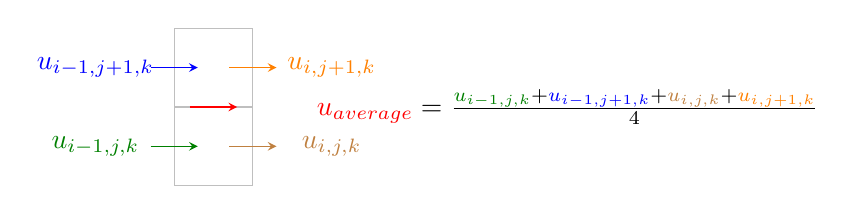
\begin{tikzpicture}
\draw[step=1cm,gray!50!white,thin] (0,0) grid (1,2);
\draw [-stealth, green!50!black] (-0.3,0.5) -- (0.3, 0.5);
\node[] at (-1, 0.5) {$\textcolor{green!50!black}{u_{i-1,j,k}}$};
\draw [-stealth, blue] (-0.3,1.5) -- (0.3, 1.5);
\node[] at (-1, 1.5) {$\textcolor{blue}{u_{i-1,j+1,k}}$};
\draw [-stealth, brown] (0.7,0.5) -- (1.3, 0.5);
\node[] at (2, 0.5) {$\textcolor{brown}{u_{i,j,k}}$};
\draw [-stealth, orange] (0.7,1.5) -- (1.3, 1.5);
\node[] at (2, 1.5) {$\textcolor{orange}{u_{i,j+1,k}}$};
\draw [-stealth, red] (0.2,1) -- (0.8, 1);
\node[] at (5, 1) {$\textcolor{red}{u_{average}}=
\frac{\textcolor{green!50!black}{u_{i-1,j,k}}+
\textcolor{blue}{u_{i-1,j+1,k}}+
\textcolor{brown}{u_{i,j,k}}+
\textcolor{orange}{u_{i,j+1,k}}}{4}
$};
\end{tikzpicture}

\caption{average of velocity} \label{velocity to other grid}
\end{figure}

\[\begin{split}
  %x velocity
  v\pdv{u}{y}&=\frac{v_{i,j-1,k}+v_{i+1,j-1,k}+v_{i,j,k}+v_{i+1,j,k}}{4}\frac{u_{i,j+1,k}-u_{i,j-1,k}}{2\Delta x}\\
  w\pdv{u}{z}&=\frac{w_{i,j,k-1}+w_{i+1,j,k-1}+w_{i,j,k}+w_{i+1,j,k}}{4}\frac{u_{i,j,k+1}-u_{i,j,k-1}}{2\Delta x}\\
  %y velocity
  u\pdv{v}{x}&=\frac{u_{i-1,j,k}+u_{i-1,j+1,k}+u_{i,j,k}+u_{i,j+1,k}}{4}\frac{v_{i+1,j,k}-v_{i-1,j,k}}{2\Delta x}\\
  w\pdv{v}{z}&=\frac{w_{i,j,k-1}+w_{i,j+1,k-1}+w_{i,j,k}+w_{i,j+1,k}}{4}\frac{v_{i,j,k+1}-v_{i,j,k-1}}{2\Delta x}\\
  %z-velocity
  u\pdv{w}{x}&=\frac{u_{i-1,j,k}+u_{i-1,j,k+1}+u_{i,j,k}+u_{i,j,k+1}}{4}\frac{w_{i+1,j,k}-w_{i-1,j,k}}{2\Delta x}\\
  v\pdv{w}{y}&=\frac{v_{i,j-1,k}+v_{i,j-1,k+1}+v_{i,j,k}+v_{i,j,k+1}}{4}\frac{w_{i,j+1,k}-w_{i,j-1,k}}{2\Delta x}\\
\end{split}
\] \label{average and partial}
We do not want to use these long equations in the code everywhere, since that would be a lot of work and unclear. Therefore, we will create a function that will calculate the partial derivative and a function that will calcute the average velocity at a point. To do this, we first need to create a struct that stores a velocity grid and the dimension of that grid.

\begin{lstlisting}[language=Rust, style=boxed, breaklines=true]
pub struct VelocityGrid{
    grid: Vec<Vec<Vec<f32>>>,
    dimension: usize,
}
\end{lstlisting}
As one can see, the grid is stored in a vector(Vec means vector). In Rust, a vector is an array that can have different sizes. Furthermore, the dimension of the array is stored as a usize, which basically is an integer with a maximum length that corresponds to the maximum length of an array. The values 0, 1 and 2 for dimension denote the x-, y-, and z-direction respectively. To prevent the use of a lot of if-statements, we create a function that can convert the dimension number to an array for which all elements, except the element corresponding to the dimension number are zero. 
\begin{lstlisting}[language=Rust, style=boxed, breaklines=true]
//Gives you the unit vector of the dimension with the given number.
//x - 0, y - 1, z - 2
fn get_dimension(dimension_number:usize)->[usize; 3]{
    let mut dim = [0,0,0];
    dim[dimension_number]=1;
    return dim;
}
\end{lstlisting}
Now we can create a function for the second order spatial derivative.
\begin{lstlisting}[language=Rust, style=boxed, breaklines=true]
fn second_order_spatial_derivative(f:&VelocityGrid, x: usize, y:usize, z:usize, dimension_number:usize) -> f32{
    let dim= get_dimension(dimension_number);
    return (f.grid[x+dim[0]][y+dim[1]][z+dim[2]] - f.grid[x-dim[0]][y-dim[1]][z-dim[2]])/(2.0*GRIDELEMENTSCALE);
}
\end{lstlisting}
Besides that, we can now also calculate the average velocity, as in figure \ref{velocity to other grid}.
\begin{lstlisting}[language=Rust, style=boxed, breaklines=true]
//This function will retrieve the velocity of an orthogonal grid a grid point of another grid.
fn get_velocity_from_orthogonal_grid(orthogonal_grid: &VelocityGrid, x:usize, y:usize, z:usize, other_grid_dimension:usize) -> f32{
    let dim_to=get_dimension(other_grid_dimension);
    let dim_from=get_dimension(orthogonal_grid.dimension);
    return 0.25*(orthogonal_grid.grid[x-dim_from[0]][y-dim_from[1]][z-dim_from[2]]//Left down
        +orthogonal_grid.grid[x-dim_from[0]+dim_to[0]][y-dim_from[1]+dim_to[1]][z-dim_from[2]+dim_to[2]]//left up
        +orthogonal_grid.grid[x][y][z]//right down
        +orthogonal_grid.grid[x+dim_to[0]][y+dim_to[1]][z+dim_to[2]]);//right up
}
\end{lstlisting}
Now we use the above two functions to write a function that calculates the convection terms \(\partial _cu\), \(\partial _cv\) and \(\partial _cw\) from equation \ref{convection terms}. We will write one function that is able to calculate all these terms: 
\begin{lstlisting}[language=Rust, style=boxed, breaklines=true]
fn convection_term(velocity_field_last_time_step: &VelocityGrid,orthogonal_velocity_field_a: &VelocityGrid, orthogonal_velocity_field_b: &VelocityGrid, x: usize, y:usize, z:usize ) -> f32{// calculate the convection term
     return DENSITY*(velocity_field_last_time_step.grid[x][y][z]*second_order_spatial_derivative(&velocity_field_last_time_step, x, y, z, velocity_field_last_time_step.dimension)
                +get_velocity_from_orthogonal_grid(&orthogonal_velocity_field_a, x, y, z, velocity_field_last_time_step.dimension)*second_order_spatial_derivative(velocity_field_last_time_step, x, y, z, orthogonal_velocity_field_a.dimension)
                +get_velocity_from_orthogonal_grid(&orthogonal_velocity_field_b, x, y, z, velocity_field_last_time_step.dimension)*second_order_spatial_derivative(velocity_field_last_time_step, x, y, z, orthogonal_velocity_field_b.dimension));
}
\end{lstlisting}




\newpage
\subsection{Discretising the diffusion term} \label{diffusion term}
Like the convection term, the diffusion term contains no temporal terms. Of course it varies, since it's terms do vary over time, but we can calculate it using information from only one timestep. We will abreviate the diffusion term of u as \(\partial _{d}u\) and the diffusion terms of v and w in a similar way\cite{MAC}. The diffusion terms of equation \ref{NSE incompressible} are\cite{MAC}:
\begin{equation}
\begin{split}
\partial _{d}u=&\eta (\pdv[2]{u}{x}+\pdv[2]{u}{y}+\pdv[2]{u}{z})\\
\partial _{d}v=&\eta (\pdv[2]{v}{x}+\pdv[2]{v}{y}+\pdv[2]{v}{z})\\
\partial _{d}w=&\eta (\pdv[2]{w}{x}+\pdv[2]{w}{y}+\pdv[2]{w}{z})\\
\end{split}
\end{equation}
We can calculate it using equation \ref{second derivative}:

\begin{lstlisting}[language=Rust, style=boxed, breaklines=true]
fn second_order_second_spatial_derivative(f: &VelocityGrid, x:usize, y:usize, z:usize, dimension_number:usize) -> f32{
    let dim = get_dimension(dimension_number);
    return(f.grid[x+dim[0]][y+dim[1]][z+dim[2]]-2.0*f.grid[x][y][z]+f.grid[x-dim[0]][y-dim[1]][z-dim[2]])/(GRIDELEMENTSCALE*GRIDELEMENTSCALE);
}
\end{lstlisting}
The sum of all three second derivatives is called the laplacian. \cite{MAC}
\begin{lstlisting}[language=Rust, style=boxed, breaklines=true]
//Laplacian velocity grid
fn laplacian(f: &VelocityGrid, x:usize, y:usize, z:usize)->f32{
    return second_order_second_spatial_derivative(f, x, y, z, 0)+second_order_second_spatial_derivative(f, x, y, z, 1)+second_order_second_spatial_derivative(f, x, y, z, 2);
}
\end{lstlisting}
So we are now able to calculate the diffusion term using:
\begin{lstlisting}[language=Rust, style=boxed, breaklines=true]
let diffusion=VISCOSITY*(laplacian(velocity_field, x, y, z));
\end{lstlisting}
We will not put this into a function just yet, because we do not know all the other terms. 
\newpage
\subsection{Discretising the pressure}
\begin{figure}[ht]
\centering
% body of the figure
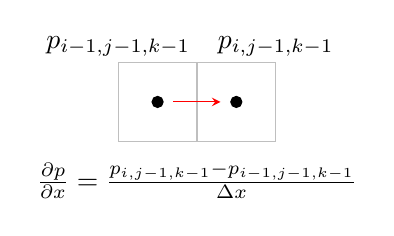
\begin{tikzpicture}
\draw[step=1cm,gray!50!white,thin] (0,0) grid (2,1);
\draw [-stealth, red] (0.7,0.5) -- (1.3, 0.5);
\filldraw[black] (0.5,0.5) circle (2pt);
\filldraw[black] (1.5,0.5) circle (2pt);
\node[] at (0, 1.2) {\(p_{i-1, j-1, k-1}\)};
\node[] at (2, 1.2) {\(p_{i, j-1, k-1}\)};
\node[] at (1, -0.5) {\(\pdv{p}{x}=\frac{p_{i, j-1, k-1}-p_{i-1, j-1, k-1}}{\Delta x}\)};

\end{tikzpicture}

\caption{derivative of pressure} \label{derivative of pressure}
\end{figure}
As in figure \ref{derivative of pressure}, we can calculate the derivatives \(\pdv{p}{x}\), \(\pdv{p}{y}\) and \(\pdv{p}{z}\)
\begin{equation}
  \begin{split}
    \pdv{p}{x}=&\frac{p_{i, j-1, k-1}-p_{i-1, j-1, k-1}}{\Delta x}\\
    \pdv{p}{y}=&\frac{p_{i-1, j, k-1}-p_{i-1, j-1, k-1}}{\Delta x}\\
    \pdv{p}{z}=&\frac{p_{i-1, j-1, k}-p_{i-1, j-1, k-1}}{\Delta x}
  \end{split}
\end{equation}
Here, (i, j, k) denotes the coordinates of the velocity in the direction we are differentiating in.  We can turn these equations into code:
\begin{lstlisting}[language=Rust, style=boxed, breaklines=true]
  fn first_order_central_spatial_pressure_derivative(f: [[[f32; PRESSUREGRIDSIZE[2]]; PRESSUREGRIDSIZE[1]]; PRESSUREGRIDSIZE[0]], x:usize, y:usize, z:usize, dimension_number:usize) -> f32{
    let position_difference=get_dimension(dimension_number);
    return (f[x+position_difference[0]][y+position_difference[1]][z+position_difference[2]]-f[x][y][z])/GRIDELEMENTSCALE;
}
\end{lstlisting}



\subsection{Implicit and explicit methods} \label{implicit and explicit}
Discretising the time can be done by using either an implicit or an explicit method.\cite{enterfea} In explicit methods, all terms except for one belong to the current timestep and the remanining term that belongs to the next timestep can be calculated easily.\cite{enterfea} In implicit methods, more variables belong to the next timestep. At first, one variable is calculated in the same way as in the explicit methods and the values of the other variables are not changed. \cite{enterfea} Thereafter, the variables  are corrected iteratively so that the solution will converge. \cite{enterfea} In the case of the incompressible Navier-Stokes equation, this means the continuity equation will converge to zero. Consequently, in explicit methods the continuity equation will always converge to zero. However, in explicit methods it is just assumed that the continuity equation holds. For the continuity equation to hold the timestep size should be very low in explicit methods. \cite{enterfea} The timestep size can be higher in implicit methods, so less timesteps are needed. \cite{enterfea} However, explicit methods do not need multiple iterations per timestep. Therefore, they compute a timestep faster.\cite{enterfea} We will use an implicit method because we intend to be able to do long simulations and they are better for larger time intervals.\cite{enterfea}


\subsection{Discretising the time}

Using the formulas for \(\partial _du\) and \(\partial _dc\) we can write equation \ref{NSE incompressible} as\cite{MAC}:
\begin{equation}
\begin{split}
  \rho \pdv{u}{t} + \partial _cu=&-\pdv{p}{x}+\partial _du + \rho g_x\\
  \rho \pdv{v}{t} + \partial _cv=&-\pdv{p}{y}+\partial _dv + \rho g_y\\
  \rho \pdv{w}{t} + \partial _cw=&-\pdv{p}{z}+\partial _dw + \rho g_z
\end{split}
\end{equation}\label{short NSE}We use this notation because it is a lot shorter. As discussed previously, we will use forward time for the derivatives. Let \(a^n\) denote $a$ in the current timestep and \(a^{n+1}\) denote a in the next timestep, where $a$ is a variable. As discussed in chapter \ref{implicit and explicit}, we will use an implicit method. We will rewrite the Navier-Stokes Equations with the spatial pressure derivative of the next timestep. This will allow us to enforce convergence. \cite{MAC}
\begin{equation}
\begin{split}
  \rho \frac{u^{n+1}-u^n}{\Delta t} + \partial _cu=&-\pdv{p^{n+1}}{x}+\partial _du + \rho g_x\\
  \rho \frac{v^{n+1}-v^n}{\Delta t} + \partial _cv=&-\pdv{p^{n+1}}{y}+\partial _dv + \rho g_y\\
  \rho \frac{w^{n+1}-w^n}{\Delta t} + \partial _cw=&-\pdv{p^{n+1}}{z}+\partial _dw + \rho g_z
\end{split}\label{time discretised NSE}
\end{equation} 
Because we are using an explicit method, we now have two variables for each formula: \(\frac{u^{n+1}-u^n}{\Delta t}\) and \(\pdv{p^{n+1}}{x}\), for x for instance. Therefore, we can not just solve this formula. We can however set the pressure term to the current pressure term and correct the error that is created in this way later. We will denote the velocities obtained in this way \(\tilde{u}\), \(\tilde{v}\) and \(\tilde{w}\)\cite{MAC}.
\begin{equation}
\begin{split}
  \rho \frac{\tilde{u}-u^n}{\Delta t} + \partial _cu=&-\pdv{p^{n}}{x}+\partial _du + \rho g_x\\
  \rho \frac{\tilde{v}-v^n}{\Delta t} + \partial _cv=&-\pdv{p^{n}}{y}+\partial _dv + \rho g_y\\
  \rho \frac{\tilde{w}-w^n}{\Delta t} + \partial _cw=&-\pdv{p^{n}}{z}+\partial _dw + \rho g_z
\end{split}\label{guess NSE}
\end{equation} 
These equations contain only one unknown variable (per equation). We can rewrite them to calculate that variable. 
\begin{equation}
  \begin{split}
  \tilde{u}=u^{n}+\frac{\Delta t}{\rho}(-\pdv{p^{n}}{x}-\partial _cu +\partial _du + \rho g_x)\\
  \tilde{v}=v^{n}+\frac{\Delta t}{\rho}(-\pdv{p^{n}}{y}-\partial _cv +\partial _dv + \rho g_y)\\
  \tilde{w}=w^{n}+\frac{\Delta t}{\rho}(-\pdv{p^{n}}{z}-\partial _cw +\partial _dw + \rho g_z)
  \end{split}\label{velocity tilde}
\end{equation} 
Now we substract equation \ref{time discretised NSE} from \ref{guess NSE}.

\begin{equation}
	\begin{split}
			%x direction
			\rho & \frac{\tilde{u} - u^{n+1}}{\Delta t} \\ &=
      \pdv{p^{n+1}}{x}-\pdv{p^{n}}{x}\\ &=
      \frac{p^{n+1}_{i,j-1,k-1}-p^{n+1}_{i-1,j-1,k-1}-(p^{n}_{i,j-1,k-1}- p^{n}_{i-1,j-1,k-1})}{\Delta x}\\
			&=-\frac{(p^{n+1}_{i-1,j-1,k-1}-p^{n}_{i-1,j-1,k-1})- 
			(p^{n+1}_{i,j-1,k-1}-p^{n}_{i,j-1,k-1})
		}{\Delta x}\\
			&=-\frac{p'_{i-1,j-1,k-1}-p'_{i,j-1,k-1}}{\Delta x}\\
% y direction
\rho & \frac{\tilde{v} - v^{n+1}}{\Delta t} \\ &= - \frac{p^{n}_{i-1,j,k-1}- p^{n+1}_{i-1,j-1,k-1}-(p^{n+1}_{i-1,j,k-1}- p^{n}_{i-1,j-1,k-1})}{\Delta x}\\
			&=-\frac{(p^{n+1}_{i-1,j-1,k-1}-p^{n}_{i-1,j-1,k-1})- 
			(p^{n+1}_{i-1,j,k-1}-p^{n}_{i-1,j,k-1})
		}{\Delta x}\\
			&=-\frac{p'_{i-1,j-1,k-1}-p'_{i-1,j,k-1}}{\Delta x}\\
%z direction
\rho & \frac{\tilde{w} - w^{n+1}}{\Delta t}  \\ &= - \frac{p^{n}_{i-1,j-1,k}- p^{n+1}_{i-1,j-1,k-1}-(p^{n+1}_{i-1,j-1,k}- p^{n}_{i-1,j-1,k-1})}{\Delta x}\\
			&=-\frac{(p^{n+1}_{i-1,j-1,k-1}-p^{n}_{i-1,j-1,k-1})-(p^{n+1}_{i-1,j-1,k}-p^{n}_{i-1,j-1,k})}{\Delta x}\\
			&=-\frac{p'_{i-1,j-1,k-1}-p'_{i-1,j-1,k}}{\Delta x}
\end{split}
\end{equation}
	Where \(p'_{i,j-1,k-1}=p^{n+1}_{i,j-1,k-1}-p^{n}_{i,j-1,k-1}\) and \(p'_{i-1,j-1,k-1}=p^{n+1}_{i-1,j-1,k-1}-p^{n}_{i-1,j-1,k-1}\).  The same is valid for the other directions. The terms denoted by p' are the pressure correction terms. We can calculate the velocity at the next timestep if we know the pressure correction:
\begin{equation}
  \begin{split}
    u^{n+1}=\tilde{u}-\frac{\Delta t}{\rho \Delta x}(p'_{i,j-1,k-1} - p'_{i-1,j-1,k-1})\\
    v^{n+1}=\tilde{v}-\frac{\Delta t}{\rho \Delta x}(p'_{i-1,j,k-1} - p'_{i-1,j-1,k-1})\\
    w^{n+1}=\tilde{w}-\frac{\Delta t}{\rho \Delta x}(p'_{i-1,j-1,k}- p'_{i-1,j-1,k-1})\\
  \end{split} \label{next timestep velocities}
\end{equation}
However, we still need to know the pressure to solve this equation. The velocity and pressure should satisfy the continuity equation (the upper equation in \ref{NSE incompressible}). We will use it to obtain the pressure.\cite{MAC}
\[
  \pdv{u}{x}+\pdv{v}{y}+\pdv{w}{z}=0
\]
We can discretise this equation for the timestep n+1 to obtain a formula for which the sole unknowns are the pressures. The pressure term has the coordinates (i,j,k)
\begin{equation}
  \begin{split}
    \frac{u^{n+1}_{i+1,j+1,k+1}-u^{n+1}_{i, j+1, k+1}}{\Delta x} + 
    \frac{v^{n+1}_{i+1,j+1,k+1}-v^{n+1}_{i+1, j, k+1}}{\Delta x} + 
    \frac{w^{n+1}_{i+1,j+1,k+1}-w^{n+1}_{i+1, j+1, k}}{\Delta x}\\=0 
  \end{split} \label{continuity discretised}
\end{equation}
We can multiply by \(\Delta x\) on both sides.
\[
  \begin{split}
    u^{n+1}_{i+1,j+1,k+1}-u^{n+1}_{i, j+1, k+1} + 
    v^{n+1}_{i+1,j+1,k+1}-v^{n+1}_{i+1, j, k+1} + 
    w^{n+1}_{i+1,j+1,k+1}-w^{n+1}_{i+1, j+1, k}\\=0 
  \end{split}
\]
Next, we fill in the velocities using equation \ref{next timestep velocities}.
\[
  \begin{split}
    \tilde{u}_{i+1,j+1,k+1} - \frac{\Delta t}{\rho \Delta x}(p'_{i+1,j,k}-p'_{i,j,k})
    -\left(\tilde{u}_{i, j+1, k+1} - \frac{\Delta t}{\rho \Delta x}(p'_{i,j,k}-p'_{i-1,j,k})\right)\\
    +\tilde{v}_{i+1,j+1,k+1} - \frac{\Delta t}{\rho \Delta x}(p'_{i,j+1,k}-p'_{i,j,k})
    -\left(\tilde{v}_{i+1, j, k+1} - \frac{\Delta t}{\rho \Delta x}(p'_{i,j,k}-p'_{i,j-1,k})\right)\\
    +\tilde{w}_{i+1,j+1,k+1} - \frac{\Delta t}{\rho \Delta x}(p'_{i,j,k+1}-p'_{i,j,k})
    -\left(\tilde{w}_{i+1, j+1, k} - \frac{\Delta t}{\rho \Delta x}(p'_{i,j,k}-p'_{i,j,k-1})\right)\\
    =0
  \end{split}
\]
We move all the pressure terms to the right hand side of the equation and keep the velocity terms at the left hand side.
\[
  \begin{split}
    \tilde{u}_{i+1,j+1,k+1}-\tilde{u}&_{i, j+1, k+1}
    +\tilde{v}_{i+1,j+1,k+1}-\tilde{v}_{i+1, j, k+1}
    +\tilde{w}_{i+1,j+1,k+1}
    -\tilde{w}_{i+1, j+1, k}\\
    &=\frac{\Delta t}{\rho \Delta x}(p'_{i+1,j,k}-p'_{i,j,k} - (p'_{i,j,k}-p'_{i-1,j,k})\\
    &+p'_{i,j+1,k}-p'_{i,j,k}-(p'_{i,j,k}-p'_{i,j-1,k})\\
    &+p'_{i,j,k+1}-p'_{i,j,k}- (p'_{i,j,k}-p'_{i,j,k-1}))\\
    =>\tilde{u}_{i+1,j+1,k+1}&-\tilde{u}_{i, j+1, k+1}
    +\tilde{v}_{i+1,j+1,k+1}-\tilde{v}_{i+1, j, k+1}
    +\tilde{w}_{i+1,j+1,k+1}
    -\tilde{w}_{i+1, j+1, k}\\
    &=\frac{\Delta t}{\rho \Delta x}(p'_{i+1,j,k} + p'_{i-1,j,k}\\
    &+p'_{i,j+1,k}+p'_{i,j-1,k}\\
    &+p'_{i,j,k+1}+p'_{i,j,k-1} - 6 p'_{i,j,k})
  \end{split}
\]
We assume that the pressure corrections for p other than (i,j,k) are zero. This will allow us to calculate the pressure correction in that point.\cite{MAC}
\[
  \begin{split}
  \tilde{u}_{i+1,j+1,k+1}&-\tilde{u}_{i, j+1, k+1}
    +\tilde{v}_{i+1,j+1,k+1}-\tilde{v}_{i+1, j, k+1}
    \\ &+\tilde{w}_{i+1,j+1,k+1}
    -\tilde{w}_{i+1, j+1, k}
     =-6\frac{\Delta t}{\rho \Delta x}p'_{i,j,k}\\
      =>p'_{i,j,k}&=-\frac{\rho \Delta x}{6\Delta t}(\tilde{u}_{i+1,j+1,k+1} \\ &-\tilde{u}_{i, j+1, k+1}
    +\tilde{v}_{i+1,j+1,k+1}-\tilde{v}_{i+1, j, k+1}
    \\ &+\tilde{w}_{i+1,j+1,k+1}
    -\tilde{w}_{i+1, j+1, k})
  \end{split}
\]
The above equation usually reaches convergence too slow, it should therefore be multiplied by a constant, \(\omega _0\).
\begin{equation}
\begin{split}
  p'_{i,j,k}&=-\omega _0\frac{\rho \Delta x}{6\Delta t}(\tilde{u}_{i+1,j+1,k+1}
  \\ &-\tilde{u}_{i, j+1, k+1}
  +\tilde{v}_{i+1,j+1,k+1}-\tilde{v}_{i+1, j, k+1}
  \\ &+\tilde{w}_{i+1,j+1,k+1}
  -\tilde{w}_{i+1, j+1, k})
\end{split} \label{pressure correction formula}
\end{equation}
Even though we multiply by \(\omega _0\), convergence is often not yet reached after one pressure correction. We therefore need to apply the pressure correction formula until convergence is reached.\cite{MAC}. 

\subsection{The algorithm}
As we have just discussed we have to apply the pressure correction formula several times, the complete algorithm is: \cite{MAC}
\paragraph{1) Initialize \(u^n\), \(v^n\), \(w^n\) and \(p^n\)} The pressure will depend on the x-coordinate due to gravity, we will write a formula to determine the initial pressure.
\paragraph{2) Predict \(\tilde{u}\), \(\tilde{v}\) and \(\tilde{w}\)} Store the results of equation \ref{velocity tilde} in new arrays, we still want to keep the last timestep velocities. 
\paragraph{3) Update boundary conditions} Implement the boundary conditions discussed in \ref{Boundary conditions and walls}.
\paragraph{4) Calculate pressure correction(p')} Store the pressure correction obtained from equation \ref{pressure correction formula} in a new array.
\paragraph{5) Update velocities to the velocities of the next timestep} Use equation \ref{next timestep velocities} to calculate the next timestep velocities. The results can be stored in the grids from step 2, because the those results are not needed anymore.
\paragraph{6) Update boundary conditions again} The boundary conditions from \ref{Boundary conditions and walls} need to be applied on the new velocity grids.
\paragraph{7) Check convergence} Check whether the continuity equation (the upper equation of \ref{NSE incompressible}) is satisfied. If it is satisfied enough, set the velocity grids created in step 1 to the velocity grids of step 5. Also, add the pressure correction grid to the pressure grid. It is now possible to go to the next timestep. If it has not converged, only add the pressure correction grid to the pressure grid and go back to step 2. The continuity equation should converge to zero after doing steps 2 till 7 multiple times. 


\subsection{The code}
\subsubsection{Programming the algorithm}
\paragraph{1) Initialize \(u^n\), \(v^n\), \(w^n\) and \(p^n\)}
\(u^n\), \(v^n\) and \(w^n\) can be set to zero or an arbitraty value. It is important that the initial condition is realistic. If it is not the program will yield weird results or it will not even converge and yield nothing at all.
\\ \\
As we have explained in \ref{The sizes of the grids} the dimensions of a velocity grid are the pressure grid size plus two in the directions orthogonal to the direction of the velocities of that grid and the pressure grid size plus one in the parallel direction. The sizes of the pressure grid will of course be PRESSUREGRIDSIZES, a constant we defined in section \ref{Constants}. We will set the initial velocities to zero. So, in code:
\begin{lstlisting}[language=Rust, style=boxed, breaklines=true]
let mut pressure_grid: [[[f32; PRESSUREGRIDSIZE[2]]; PRESSUREGRIDSIZE[1]]; PRESSUREGRIDSIZE[0]]=[[[0.0; PRESSUREGRIDSIZE[2]]; PRESSUREGRIDSIZE[1]]; PRESSUREGRIDSIZE[0]];//pressureGrid[x][y][z] is the pressure at coordinates (x,y,z)
    let mut velocity_x = VelocityGrid{grid: vec![vec![vec![0.0;PRESSUREGRIDSIZE[2]+2]; PRESSUREGRIDSIZE[1]+2]; PRESSUREGRIDSIZE[0]+1], dimension:0};// z,y,x !!!
    let mut velocity_y = VelocityGrid{grid: vec![vec![vec![0.0;PRESSUREGRIDSIZE[2]+2]; PRESSUREGRIDSIZE[1]+1]; PRESSUREGRIDSIZE[0]+2], dimension:1}; 
    let mut velocity_z = VelocityGrid{grid: vec![vec![vec![0.0;PRESSUREGRIDSIZE[2]+1]; PRESSUREGRIDSIZE[1]+2]; PRESSUREGRIDSIZE[0]+2], dimension:2}; 
    
\end{lstlisting}
Here the pressure is set to zero, which it should not be, since there is no vacuum. To determine the initial pressure we need to take gravity into account. The mass of fluid layers above a certain layer will exercise pressure on that layer. The pressure can be determined using the following formula:
\[
\begin{split}
p(h)&=\frac{F}{A}=\frac{F_{atmospheric}+F_{g,water}}{A}
\\&=\frac{F_{atmospheric}}{A}+\frac{\rho V_{water}g}{A}
\\&=p_{atmospheric}+\rho hg
\end{split}
\]
Where h is the height. z=0 is the bottom, so:
\[
\begin{split}
  h&=z_{max}-z\\
  &=>p(z)=p_{atmospheric}+\rho g(z_{max}-z)
\end{split}
\]
We can use this function to create the desired pressure function:
\begin{lstlisting}[language=Rust, style=boxed, breaklines=true]
fn initialize_pressure_grid(pressure_grid: &mut [[[f32; PRESSUREGRIDSIZE[2]];PRESSUREGRIDSIZE[1]];PRESSUREGRIDSIZE[0]]){
    for x in 0..(PRESSUREGRIDSIZE[0]-1){//velocty_grid has PRESSUREGRIDSIZE[dimension] elements, so loop from 0 to PRESSUREGRIDSIZE[dimension]-1.
        for y in 0..(PRESSUREGRIDSIZE[1]-1){
            for z in 0..(PRESSUREGRIDSIZE[2]-1){
                //The pressure should be the atmosferic pressure(101,325Pa) plus the pressure that is exercised by the water above a point on the water at that point. 
                pressure_grid[x][y][z]=ATMOSPHERIC_PRESSURE+DENSITY*(PRESSUREGRIDSIZE[2] as f32 - z as f32)*GRIDELEMENTSCALE*EXTERNALFORCE[2];
            }
        }
    }
}
\end{lstlisting}



\paragraph{2) Predict \(\tilde{u}\), \(\tilde{v}\) and \(\tilde{w}\)}  We start with formula \ref{velocity tilde}:

\begin{lstlisting}[language=Rust, style=boxed, breaklines=true]
fn predict_velocity(provisonal_velocity_field: &mut VelocityGrid, velocity_field_last_time_step: &VelocityGrid, orthogonal_velocity_field_a: &VelocityGrid, orthogonal_velocity_field_b: &VelocityGrid, pressure_grid: [[[f32; PRESSUREGRIDSIZE[2]]; PRESSUREGRIDSIZE[1]]; PRESSUREGRIDSIZE[0]]){
    let dim=get_dimension(provisonal_velocity_field.dimension);
    for x in 1..(PRESSUREGRIDSIZE[0]-dim[0]+1) {
        for y in 1..(PRESSUREGRIDSIZE[1]-dim[1]+1) {
            for z in 1..(PRESSUREGRIDSIZE[2]-dim[2]+1) {
                //Diffusion term
                let diffusion=VISCOSITY*(laplacian(velocity_field_last_time_step, x, y, z));
                //And finally, the provisional velocity
                provisonal_velocity_field.grid[x][y][z]=velocity_field_last_time_step.grid[x][y][z]+TIMESTEPSIZE/DENSITY*(-convection_term(velocity_field_last_time_step, orthogonal_velocity_field_a, orthogonal_velocity_field_b, x, y, z)-first_order_central_spatial_pressure_derivative(pressure_grid, x-1, y-1, z-1, velocity_field_last_time_step.dimension)+diffusion+DENSITY*EXTERNALFORCE[velocity_field_last_time_step.dimension]);
            }
        }
    }

}
\end{lstlisting}
The function above stores the provisional velocities obtained from equation \ref{velocity tilde} in provisional\_velocity\_field, which is a seperate grid. The diffusion term is calculated as in chapter \ref{diffusion term}.

\paragraph{3) Update boundary conditions}
Ideally, the user can set the boundary conditions themselves. Although this is currently possible, it requires the user to perform quite a lot of programming work themselves. We will create a few functions the user can use to set the boundary conditions. 
\\ \\
We will enforce a no-slip boundary condition at the wall as we have discussed in section \ref{Boundary conditions and walls}. We will first create a function that will enforce that boundary condition in the orthogonal direction. 
\begin{lstlisting}[language=Rust, style=boxed, breaklines=true]
/Set the orthogonal velocity to a certain value on a wall
fn set_orthogonal_boundary_condition_at_wall(orthogonal_velocity_grid: &mut VelocityGrid, min_coords: [usize; 3], max_coords: [usize; 3], value: f32){
    for x in min_coords[0]..=max_coords[0]{
        for y in min_coords[1]..=max_coords[1]{
            for z in min_coords[2]..=max_coords[2]{
                orthogonal_velocity_grid.grid[x][y][z]=value;
            }
        }
    }
}
\end{lstlisting}
This function will set the orthogonal boundary condition for a rectangular wall with given minimum and maximum coordinates. As one can see, we have use ..= instead of .. in the for loops. We have done this because we also want to set the boundary condition at the maximum coordinates. This way, the boundary condition will also be set when one component of the minimum coordinates is equal to the same  component of the maximum coordinates. The user can choose the variable value, so that he or she can create inflows and outflows by setting it to a nonzero value. When value is zero there is no flow.
\\ \\
We also have to enforce the boundary values in the directions parallel to the wall, again using the formulas from section \ref{Boundary conditions and walls}. This is a little bit trickier, because we have to use neighboring points. The user will have to specify whether the given points are on the side of the wall with lower coordinates or higher coordinates.
\begin{lstlisting}[language=Rust, style=boxed, breaklines=true]
//wall_is_on_lower_side=0 means the wall is on the side with lower coordinates seen from the dry side and wall_is_on_lower_side=1 means the wall is on the side with higher coordinates. 
//orthogonal_dimension is the dimension number(0 for x, 1 for y, 2 for z) of the dimension orthogonal to the wall
fn set_parallel_boundary_condition_at_wall(parallel_velocity_grid: &mut VelocityGrid, min_coords: [usize; 3], max_coords: [usize; 3], wall_is_on_lower_side: bool, orthogonal_dimension: usize){
    let dim=get_dimension(orthogonal_dimension);
    let transformation_in_one_dimension=1 - 2 * (wall_is_on_lower_side as isize);// -1 when a lower element is needed, +1 when a higher element is needed
    let transformation_to_neighbor:[isize; 3]=[(dim[0] as isize) * transformation_in_one_dimension, (dim[1] as isize) * transformation_in_one_dimension, (dim[2] as isize) * transformation_in_one_dimension];// This is the transformation to the neighbor opposite of the wall
    for x in min_coords[0]..=max_coords[0]{
        for y in min_coords[1]..=max_coords[1]{
            for z in min_coords[2]..=max_coords[2]{
                //The parallel velocity should be the opposite of the parallel velocity on the other side of the wall, so that the average is zero.
                parallel_velocity_grid.grid[x][y][z]=-parallel_velocity_grid.grid[(x as isize + transformation_to_neighbor[0])as usize][(y as isize + transformation_to_neighbor[1]) as usize][(z as isize+transformation_to_neighbor[2]) as usize];          
            }
        }
    }
}
\end{lstlisting}
To make using the program a little bit easier, we have created a function that sets the boundary conditions for two walls, it is explained in the comments.
\begin{lstlisting}[language=Rust, style=boxed, breaklines=true]
fn set_boundary_conditions_of_two_parallel_walls(orthogonal_velocity_grid: &mut VelocityGrid, parallel_velocity_grid_a: &mut VelocityGrid, parallel_velocity_grid_b: &mut VelocityGrid, orthogonal_velocity_grid_value: f32){
    let dim= get_dimension(orthogonal_velocity_grid.dimension);
    //Set the max positions, the position coordinate orthogonal to the wall will be set to zero later
    let mut max_orthogonal_coords=[PRESSUREGRIDSIZE[0]+1, PRESSUREGRIDSIZE[1]+1, PRESSUREGRIDSIZE[2]+1];//max coordinates for orthogonal velocities  
    let mut max_parallel_coords=PRESSUREGRIDSIZE;//Max coordinates for parallel velocities
    //The coordinates of one wall have coordinate zero in one dimension
    max_orthogonal_coords[orthogonal_velocity_grid.dimension]=0;//Take the wall that has the 0 coordinate in one direction
    max_parallel_coords[orthogonal_velocity_grid.dimension]=0;// The sizes of the parallel grids are the same in the other dimensions, so we will loop through the same values.
    //Set boundary conditions for the zero wall
    set_orthogonal_boundary_condition_at_wall(orthogonal_velocity_grid, [0,0,0], max_orthogonal_coords, orthogonal_velocity_grid_value);
    set_parallel_boundary_condition_at_wall(parallel_velocity_grid_a, [0,0,0], max_parallel_coords, false, orthogonal_velocity_grid.dimension);
    set_parallel_boundary_condition_at_wall(parallel_velocity_grid_b, [0,0,0], max_parallel_coords, false, orthogonal_velocity_grid.dimension);
    //The other wall has one coordinate at the maximum, so set that coordinate to the maximum
    max_orthogonal_coords[orthogonal_velocity_grid.dimension]=PRESSUREGRIDSIZE[orthogonal_velocity_grid.dimension];
    max_parallel_coords[orthogonal_velocity_grid.dimension]=PRESSUREGRIDSIZE[orthogonal_velocity_grid.dimension]+1;
    let minimum_parallel_coords=[(PRESSUREGRIDSIZE[0]+1)*dim[0], (PRESSUREGRIDSIZE[1]+1)*dim[1], (PRESSUREGRIDSIZE[2]+1)*dim[2]];
    let minimum_orthogonal_coords=[PRESSUREGRIDSIZE[0]*dim[0],PRESSUREGRIDSIZE[1]*dim[1], PRESSUREGRIDSIZE[2]*dim[2]];
    //Set boundary conditions for the maximum wall
    set_orthogonal_boundary_condition_at_wall(orthogonal_velocity_grid, minimum_orthogonal_coords, max_orthogonal_coords, orthogonal_velocity_grid_value);
    set_parallel_boundary_condition_at_wall(parallel_velocity_grid_a, minimum_parallel_coords, max_parallel_coords, true, orthogonal_velocity_grid.dimension);
    set_parallel_boundary_condition_at_wall(parallel_velocity_grid_b, minimum_parallel_coords, max_parallel_coords, true, orthogonal_velocity_grid.dimension);
    

}
\end{lstlisting}
We would like to implement more options for modifying boundary conditions in the future, Unfortunately, this is beyond the scope of this project.

\paragraph{4) Calculate pressure correction(p')}

Next, we turn equation \ref{pressure correction formula} into code. 
\begin{lstlisting}[language=Rust, style=boxed, breaklines=true]
fn calculate_pressure_correction(x_velocity: & VelocityGrid, y_velocity: & VelocityGrid, z_velocity: & VelocityGrid)->[[[f32; PRESSUREGRIDSIZE[2]]; PRESSUREGRIDSIZE[1]]; PRESSUREGRIDSIZE[0]]{
    let mut pressure_correction: [[[f32; PRESSUREGRIDSIZE[2]]; PRESSUREGRIDSIZE[1]]; PRESSUREGRIDSIZE[0]]=[[[0.0; PRESSUREGRIDSIZE[2]]; PRESSUREGRIDSIZE[1]]; PRESSUREGRIDSIZE[0]];//Here we will store the pressure corrections.
    let constant_term_pressure_equation=RELEXATION*DENSITY*GRIDELEMENTSCALE/(6.0*TIMESTEPSIZE);//The lower part of the equation is this constant.
        for i in 0..PRESSUREGRIDSIZE[0] - 1{
            for j in 0..PRESSUREGRIDSIZE[1] - 1{
                for k in 0..PRESSUREGRIDSIZE[2] - 1{
                    pressure_correction[i][j][k]=-constant_term_pressure_equation*(x_velocity.grid[i+1][j+1][k+1] - x_velocity.grid[i][j+1][k+1]+ y_velocity.grid[i+1][j+1][k+1] - y_velocity.grid[i+1][j][k+1] + z_velocity.grid[i+1][j+1][k+1]-z_velocity.grid[i+1][j+1][k]);
                }
            }
        }
    return pressure_correction;
}
\end{lstlisting}

\paragraph{5) Update velocities to the velocities of the next timestep} 
We also write a function for equation \ref{next timestep velocities}. We do not need the provisional velocities anymore, so we will store the new velocities in the provisional velocity array for storage efficiency.

\begin{lstlisting}[language=Rust, style=boxed, breaklines=true]
fn update_velocity_field(velocity_field: &mut VelocityGrid, pressure_correction : &[[[f32; PRESSUREGRIDSIZE[2]]; PRESSUREGRIDSIZE[1]]; PRESSUREGRIDSIZE[0]]){
    let dim=get_dimension(velocity_field.dimension);
    let constant_term_velocity_equation=TIMESTEPSIZE/(DENSITY*GRIDELEMENTSCALE);
    for i in 1..PRESSUREGRIDSIZE[0]+1-dim[0]{
        for j in 1..PRESSUREGRIDSIZE[1]+1-dim[1]{
            for k in 1..PRESSUREGRIDSIZE[2]+1-dim[2]{
                velocity_field.grid[i][j][k]=velocity_field.grid[i][j][k]-constant_term_velocity_equation*(pressure_correction[i+dim[0]-1][j+dim[1]-1][k+dim[2]-1]- pressure_correction[i-1][j-1][k-1]);
            }
        }
    }
}
\end{lstlisting}
\paragraph{6) Update boundary conditions again}
This is the same as step 3, it is important that the same boundary conditions are enforced
\paragraph{7) Check convergence}
The velocities should satisfy the continuity equation (the upper equation of \ref{NSE incompressible}). As we have seen the discretised version of the continuity equation is \ref{continuity discretised}. Because we have discretised the equations, the continuity equation will not be completely satisfied. However, after each pressure correction the continuity equation should converge to zero a little more. We will stop correcting the pressure when the error is smaller than the constant ALLOWEDERROR. Calculating the error is very easy, since it is just the sum of the derivatives of the velocities in their own direction. We will calulate the derivatives for a pressure point and use central derivatives, so that all three derivatives are calculable. So we first need to define that derivative:

\begin{lstlisting}[language=Rust, style=boxed, breaklines=true]
fn first_order_central_spatial_derivative(f: &VelocityGrid, x: usize, y: usize, z:usize)->f32{//practically identical to first_order_forward_spatial_derivative, but for clarity we keep it.
    let dim=get_dimension(f.dimension);
    return (f.grid[x+dim[0]][y+dim[1]][z+dim[2]]-f.grid[x][y][z])/GRIDELEMENTSCALE;
}
\end{lstlisting}
Now we can create a function that determines whether the error is too big somewhere:
\begin{lstlisting}[language=Rust, style=boxed, breaklines=true]
fn check_convergence(provisional_velocity_x:&VelocityGrid, provisional_velocity_y: &VelocityGrid, provisional_velocity_z: &VelocityGrid)->bool{
    
    for x in 0..PRESSUREGRIDSIZE[0]{
        for y in 0..PRESSUREGRIDSIZE[1]{
            for z in 0..PRESSUREGRIDSIZE[2]{
                let error=first_order_central_spatial_derivative(&provisional_velocity_x, x, y, z)
                    +first_order_central_spatial_derivative(&provisional_velocity_y, x, y, z)
                    +first_order_central_spatial_derivative(&provisional_velocity_z, x, y, z);    
                if error.abs()>ALLOWEDERROR{
                    println!("Convergence not yet reached, error is {} at ({}, {}, {})", error, x, y, z );
                    return false;

                }
            }
        }
    } 
    return true;
}
\end{lstlisting}

\subsubsection{Switching grids}
We want to display the velocities on a collocated grid and not on a staggered grid, therefore we will create a function that calculates the velocities at pressure points:

\begin{lstlisting}[language=Rust, style=boxed, breaklines=true]
fn get_velocity_at_pressure_point(velocity_grid: &VelocityGrid, x: usize, y: usize, z: usize)->f32{
    let dim= get_dimension(velocity_grid.dimension);
    return velocity_grid.grid[x+1][y+1][x+1]-velocity_grid.grid[x+1-dim[0]][y+1-dim[1]][z+1-dim[2]];//Just take the average
}
\end{lstlisting}
This function just takes the average of the two nearest velocity points. Using this function we can get all velocity components at every pressure point. However, if we visualise all velocity components of a large grid we will show so much data that one can not interpret it well. Therefore, we want to be able to scale down the resolution. We will do that using the following function:
\begin{lstlisting}[language=Rust, style=boxed, breaklines=true]
//Calculates the interval between the velocities that should be shown in one dimension
fn calc_step_size(from_dimension: usize, to_dimension: usize)->usize{
    return from_dimension/to_dimension;
} 
\end{lstlisting}
The function divides a usize by a usize. A usize is an integer and thus Rust wants the answer to be an integer as well. Rust will therefore round it down when it is not an integer. We want this to happen because the array elements are all integers. Furthermore, when the answer is rounded down there will be no out-of-bounds errors. 
\\ \\
We can use these functions to convert the velocities to a collocated grid and visualise them:
\begin{lstlisting}[language=Rust, style=boxed, breaklines=true]
//min_coords and max_coords are the pressure coordinates of which we want to know the velocities(this function will determine those velocities by taking the average of nearby velocities)
//data_grid_point_size is the size of the grid we want to show to the user
pub fn convert_velocities_to_collocated_grid_and_visualise(min_coords: [usize; 3], max_coords: [usize;3], data_grid_point_size: [usize; 3], velocity_grid_x: &VelocityGrid, velocity_grid_y: &VelocityGrid, velocity_grid_z: &VelocityGrid) -> Vec<Vec<Vec<[f32;3]>>>{
    let step_size=[calc_step_size(max_coords[0]-min_coords[0], data_grid_point_size[0]), calc_step_size(max_coords[1]-min_coords[1], data_grid_point_size[1]), calc_step_size(max_coords[2]-min_coords[2], data_grid_point_size[2])];
    let mut return_data: Vec<Vec<Vec<[f32; 3]>>>=vec![vec![vec![[0.0; 3]; data_grid_point_size[0]]; data_grid_point_size[1]]; data_grid_point_size[0]];
    for x in 0..data_grid_point_size[0]{
        for y in 0..data_grid_point_size[1]{
            for z in 0..data_grid_point_size[2]{
                return_data[x][y][z]=[get_velocity_at_pressure_point(&velocity_grid_x, x*step_size[0], y*step_size[1], z*step_size[2]),  get_velocity_at_pressure_point(&velocity_grid_y, x*step_size[0], y*step_size[1], z*step_size[2]), get_velocity_at_pressure_point(&velocity_grid_z, x*step_size[0], y*step_size[1], z*step_size[2])];
            }
        }
    }
    return return_data;
}
\end{lstlisting}

\subsubsection{Putting it all together}
Using the functions from previous chapters, we can finally create a function for one timestep:
\begin{lstlisting}[language=Rust, style=boxed, breaklines=true]
fn simulation_time_step(velocity_grid_x: &mut VelocityGrid, velocity_grid_y: &mut VelocityGrid, velocity_grid_z: &mut VelocityGrid,  pressure_grid: &mut [[[f32; PRESSUREGRIDSIZE[2]];PRESSUREGRIDSIZE[1]];PRESSUREGRIDSIZE[0]], time_step: i32) -> Vec<Vec<Vec<[f32;3]>>>{
    let i:&mut i32=&mut 0;
    while *i<MAXITERATIONSPERTIMEFRAME {
        //1) Predict u, v and w,
        let mut provisional_velocity_x = VelocityGrid{grid: vec![vec![vec![0.0;PRESSUREGRIDSIZE[2]+2]; PRESSUREGRIDSIZE[1]+2]; PRESSUREGRIDSIZE[0]+1], dimension:0};
        let mut provisional_velocity_y = VelocityGrid{grid: vec![vec![vec![0.0;PRESSUREGRIDSIZE[2]+2]; PRESSUREGRIDSIZE[1]+1]; PRESSUREGRIDSIZE[0]+2], dimension:1}; 
        let mut provisional_velocity_z = VelocityGrid{grid: vec![vec![vec![0.0;PRESSUREGRIDSIZE[2]+1]; PRESSUREGRIDSIZE[1]+2]; PRESSUREGRIDSIZE[0]+2], dimension:2}; 
    
        //x-velocity
        predict_velocity(&mut provisional_velocity_x, &velocity_grid_x, &velocity_grid_y, &velocity_grid_z, *pressure_grid);
        //y-velocity
        predict_velocity(&mut provisional_velocity_y, &velocity_grid_y, &velocity_grid_x, &velocity_grid_z, *pressure_grid);
        //z-velocity
        predict_velocity(&mut provisional_velocity_z, &velocity_grid_z, &velocity_grid_x, &velocity_grid_y, *pressure_grid);
        
        //2)Update boundary conditions(i.e. set walls)
        set_wall_boundary_conditions( &mut provisional_velocity_x,  &mut provisional_velocity_y,  &mut provisional_velocity_z, 1.0, time_step);

        //3)Calculate pressure correction
        let mut pressure_correction: [[[f32; PRESSUREGRIDSIZE[2]]; PRESSUREGRIDSIZE[1]]; PRESSUREGRIDSIZE[0]]=calculate_pressure_correction(&provisional_velocity_x, &provisional_velocity_y, &provisional_velocity_z);
    

        //4)Update u and v
        update_velocity_field(&mut provisional_velocity_x, &pressure_correction);
        update_velocity_field(&mut provisional_velocity_y, &pressure_correction);
        update_velocity_field(&mut provisional_velocity_z, &pressure_correction);
        
        //5)Update boundary values
        set_wall_boundary_conditions( &mut provisional_velocity_x,  &mut provisional_velocity_y,  &mut provisional_velocity_z, 1.0, time_step);
        
        //6)Check convergence
        if check_convergence(&provisional_velocity_x, &provisional_velocity_y, &provisional_velocity_z) {// If the continuity equation has converged we can go to the next timestep
            velocity_grid_x.grid=provisional_velocity_x.grid.clone();
            velocity_grid_y.grid=provisional_velocity_y.grid.clone();
            velocity_grid_z.grid=provisional_velocity_z.grid.clone();
            *i=MAXITERATIONSPERTIMEFRAME;
        }else{
            println!{"convergence has not yet been reached, trying again, iteration: {}", i};
            if *i+1==MAXITERATIONSPERTIMEFRAME{//If the continuity equation has not converged after many iterations something probably went wrong. Therefore the program will have to be terminated then.
                println!("Last iteration {} did not converge", i);
                std::process::exit(1);
            }
            
        }
        *i=*i+1;
        println!("i is {}", i);
        //7) Update pressure
        update_pressure(pressure_grid, &pressure_correction);
    }  
    println!("Finished! At (2,2,2) velocity is ({}, {}, {})",velocity_grid_x.grid[2][2][2], velocity_grid_y.grid[2][2][2],velocity_grid_z.grid[2][2][2]);
    return convert_velocities_to_collocated_grid_and_visualise([1,1,1], [PRESSUREGRIDSIZE[0]-1, PRESSUREGRIDSIZE[1]-1, PRESSUREGRIDSIZE[2]-1], [4,4,4], velocity_grid_x, velocity_grid_y, velocity_grid_z);
}
\end{lstlisting}
The renderer will then show these results, thereafter we can move to the next timestep.








\newpage  
\section{Visualisation} \label{Visualisation}
\subsection{Drawing}
The way we decided to show the movement of the fluids is by drawing arrows in a space of three dimensions. We do this by first loading in the arrow from an OBJ file. An OBJ file is the simplest way of storing three dimensional objects. We define the center of the arrow as (0,0,0). This makes rotation and translation easier. We also make sure that by default the arrow position is up, giving us the vector $\vec{v}=(0,0,1)$. We then create multiple instances of that arrow which we multiply with a quaternion that is the cross product of the desired rotation and the neutral rotation and we set the scalar equal to the distance between the endpoints of the vectors with the origin as a starting point. finally we transform the arrow by a vector $\vec{x}=(x,y,z)$, giving us the following transformation: 
$\begin{bmatrix}
1 & 0 & 0 & 0\\
0 & 1 & 0 & 0\\
0 & 0 & 1 & 0\\
x & y & z & 1
\end{bmatrix}$. Due to the z-component in computer graphics being defined as the distance from the screen and the height as the y-component, we also need to switch the z and y-components.$\begin{bmatrix}
1 & 0 & 0 & 0\\
0 & 0 & 1 & 0\\
0 & 1 & 0 & 0\\
x & y & z & 1
\end{bmatrix}$
The final multiplication matrix then becomes: 
$\begin{bmatrix}

d & 0 & y & -x\\
0 & d & x & y\\
-y & -x & d & 0\\
xd-zy+x & yd -zx - y & 2xy + zd & -x^2 + y^2 + d 

\end{bmatrix}$
where $d = ||\vec{x}-\vec{v}||$.\cite{Quaternion rotation}
\subsection{Data capturing}
In order to actually show the data, we need to draw the arrows by defining the vertices that make up the arrows. We then multiply it with the transformation matrix from the previous chapter and finally with a standard camera matrix. \cite{mvp} Then to get the final image we create a lot of instances of that arrow which are rotated and translated with the transformation matrix of the previous chapter. \label{Drawing} We finally define a grid by drawing lines with a start and endpoint multiplied with the camera matrix.
%TODO: add image

\newpage
\section{Conclusion} \label{Conclusion}
\subsection{Results}
The final result looks something like this:
\begin{figure}[h]
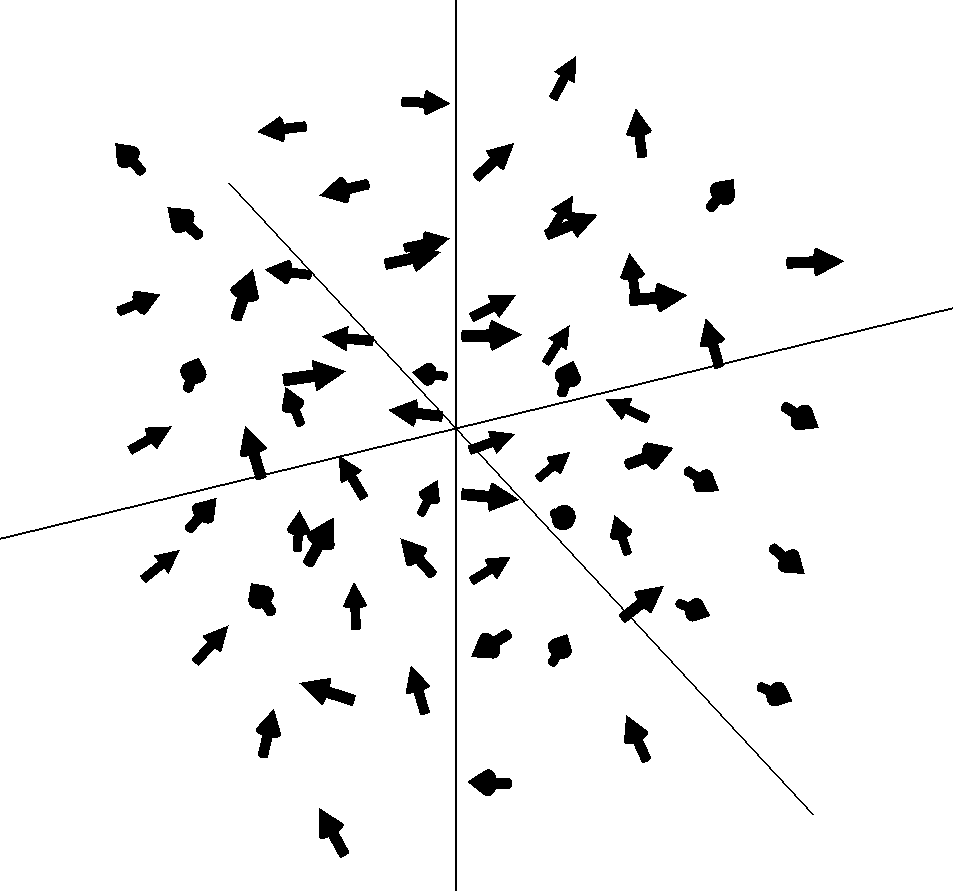
\includegraphics[width=\textwidth]{result1}
\centering
\caption{The situation after a few timesteps with inflow and outflow}
\end{figure}
\\ \\
We were quite content with this result despite the fact that it was not perfect. We had a reasonably well working simulation albeit with some limitations and speed issues. When simulating a relatively small grid, it worked quite well but when using a larger grid, things started to get pretty slow. To work around this issue we decided to only use relatively small grids to test the simulation.
\subsection{Discussion}
Although we have a working prototype, it is really just that, a prototype. The simulation works but there is a slight deviation in the continuity equation that increases slightly every timestep. The rendering part is also nowhere near perfect, the arrows are sometimes a bit hard to see and the camera is quite limited. But the worst issues are most definitively performance and memory usage, simulating a small grid is not really an issue but when you go over 50 x 50 x 50 you can expect to wait up to a minute per timestep on even a reasonably fast system. This can be reduced significantly by increasing the maximum allowed deviation but this of course comes at the cost of accuracy. Another issue is memory usage, each point in the grid requires the velocity and pressure to be stored requiring 4 numbers of each 4 bytes in size which means the amount of memory required in a square grid is $16*size^3$ which means a grid of $1000^3$ uses 16Gb in the ideal case. In reality, temporary variables, the rendering and overhead increase this number even more. If we had more time for this project we would have implemented more discretization methods and in the ideal case we would have used something like Vulkan compute or CUDA to perform many calculations in parallel instead of in series. Furthermore, we would have liked to give users options to set and edit boundary conditions. Currently, the only way to do this is by changing the boundary condition function itself, which requires that one recompiles the code.
\newpage
%Eind PWS, start bronnenlijst
\begin{thebibliography}{3}
\bibitem{Discretization types}
\url{https://resources.pcb.cadence.com/blog/2020-cfd-simulation-types-discretization-approximation-and-algorithms}
\bibitem{What is discretization}
\url{https://www.manchestercfd.co.uk/post/what-is-discretization}
\bibitem{Difference equation}
\url{https://www.britannica.com/science/difference-equation}
\bibitem{Taylor series}
\url{https://courses.engr.illinois.edu/cs357/fa2019/assets/lectures/Lecture8-Sept19.pdf}
\bibitem{Navier_Stokes_afleiding}
\url{https://web.iit.edu/sites/web/files/departments/academic-affairs/academic-resource-center/pdfs/Navier_Stokes.pdf}
\bibitem{Fluid simulation methods}
\url{https://www.dive-solutions.de/articles/cfd-methods}
\bibitem{Lattice Boltzmann implementation}
\url{https://arxiv.org/pdf/cs/0501021.pdf}
\bibitem{Taylor series approximation}
\url{https://brilliant.org/wiki/taylor-series-approximation/}
\bibitem{quantstart FDM}
\url{https://www.quantstart.com/articles/Derivative-Approximation-via-Finite-Difference-Methods/}
\bibitem{Big O}
\url{https://math.stackexchange.com/questions/501735/why-do-we-use-big-oh-in-taylor-series}
\bibitem{Maxwell FDM}
\url{https://maxwell.ict.griffith.edu.au/jl/Chapter5.pdf}
\bibitem{Boundary Element Method}
\url{https://pure.tue.nl/ws/files/3372975/696955.pdf}
\bibitem{Finite Element Method}
\url{https://www.comsol.com/multiphysics/finite-element-method}
\bibitem{Finite Volume}
\url{https://link.springer.com/chapter/10.1007\%2F978-3-319-16874-6\_19}
\bibitem{More_FDM}
\url{http://www.fem.unicamp.br/~phoenics/SITE_PHOENICS/Apostilas/CFD-1_U\%20Michigan_Hong/Lecture13.pdf}
\bibitem{no-slip boundary condition}
\url{https://www.quora.com/What-is-the-physics-behind-no-slip-condition-in-fluid-mechanics}
\bibitem{free slip boundary condition}
\url{https://physics.stackexchange.com/questions/383096/understanding-free-slip-boundary-condition}
%Begin of Navier-Stokes
\bibitem{Navier Stokes incompressible}
\url{https://www.tec-science.com/mechanics/gases-and-liquids/derivation-of-the-navier-stokes-equations/}
\bibitem{Stresses}
\url{https://www.paramvisions.com/2021/04/what-is-normal-stress-shear-stress.html}
\bibitem{Navier Stokes compressible}
\url{http://ingforum.haninge.kth.se/armin/fluid/exer/deriv_navier_stokes.pdf}
%Neglections
\bibitem{NSE features}
\url{https://projects.iq.harvard.edu/files/ac274_2015/files/lecture2_3.pdf}
\bibitem{Viscosity}
\url{https://physics.info/viscosity/}
\bibitem{Dissipation}
\url{https://www.tec-science.com/thermodynamics/thermodynamic-processes-in-closed-systems/what-is-meant-by-dissipation-of-energy/}
\bibitem{Turbulence}
\url{https://www.simscale.com/blog/2017/12/turbulence-cfd-analysis/}
\bibitem{Steady and unsteady}
\url{http://www.nzdl.org/cgi-bin/library?e=d-00000-00---off-0hdl--00-0----0-10-0---0---0direct-10---4-------0-1l--11-en-50---20-about---00-0-1-00-0--4----0-0-11-10-0utfZz-8-00\&cl=CL1.11\&d=HASH011f05bf8734d88d1a080257.12.1\&gt=1}
\bibitem{NASA NSE}
\url{https://www.grc.nasa.gov/WWW/k-12/airplane/nseqs.html}
%End of Navier Stokes
%Projection method
\bibitem{Staggered grid}
\url{https://www.youtube.com/watch?v=Kf_RHzaqFBc}
\bibitem{MAC}
\url{https://www.youtube.com/watch?v=0qtvRjuTihY}
\bibitem{enterfea}
\url{https://enterfea.com/implicit-vs-explicit/}
\bibitem{Vulkan}
https://vulkan-tutorial.com/
\bibitem{visual room}
\url{http://thevisualroom.com/marker_and_cell_method.html}
\bibitem{Quaternion rotation}
\url{https://stackoverflow.com/questions/1171849/finding-quaternion-representing-the-rotation-from-one-vector-to-another}
\bibitem{mvp}
\url{https://www.youtube.com/watch?v=x_Ph2cuEWrE}
\bibitem{Millenium Problems}
\url{https://www.claymath.org/millennium-problems}
\bibitem{Rust}
\url{https://www.rust-lang.org/}
\end{thebibliography}
\end{document}